\documentclass{article}
\usepackage{graphicx}

\usepackage{titling}
\newcommand{\subtitle}[1]{%
  \posttitle{%
    \par\end{center}
    \begin{center}\large#1\end{center}
    \vskip0.5em}%
}

\begin{document}

\title{Software Entwicklung Projekt - Sonjas Coursera - Use Case Diagramm}
\subtitle{Allgemeine Informatik - IN7 - Prof. Dr. Jobst}
\author{Sonja Riethig}

\maketitle

\begin{abstract}
Das Projekt "Sonjas Coursera" implementiert einen einfachen Online-Kurs - Anbieter. Im Folgenden werden die Anforderungen an das Projekt mithilfe von Diagrammen mit Anmerkungen dargestellt.
\end{abstract}

\newpage

\section{Use Case Diagramm}

\begin{figure}[!h]
    \centering
    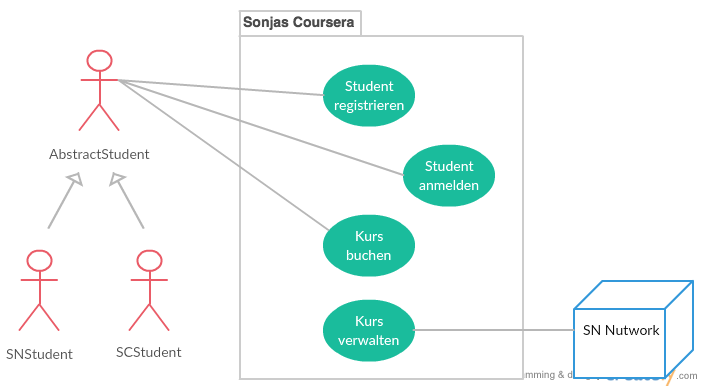
\includegraphics[width=15cm]{../images/SonjasCoursera-UseCaseDiagram.png}
    \caption{Use Case Diagramm}
    \label{Use Case Diagramm}
\end{figure}

\section{Details der Use Cases}

\subsection{Student registrieren}

\begin{itemize}
\item ein User kann sich mit Email und Passwort registrieren
\item ein User, der sich mit Email und Passwort registriert, muss seine persönlichen Daten und Adressdaten eingeben
\end{itemize}

\begin{itemize}
\item ein User, der bereits einen Account beim Partnerprojekt Nutwork besitzt, kann sich mit dem Nutzernamen und Passwort seines Nutwork-Accounts registrieren
\item ein User, der sich mit seinem Nutwork-Account registriert, muss sein persönlichen Daten ggf. \"andern und best\"atigen
\item ein User, der sich mit seinem Nutwork-Account registriert, muss seine Adressdaten eingeben
\end{itemize}

\subsection{Student anmelden}

\begin{itemize}
\item ein registrierter User kann sich mit Email und Passwort anmelden
\item ein User, der \"uber Nutwork registriert ist, kann sich mit Nutzernamen und Passwort seines Nutwork-Accounts anmelden
\item nach der Anmeldung kann der User sein Profil (d.h. seine Daten, seine gebuchten Kurse und eine \"Ubersicht aller verf\"ugbaren Kurse) einsehen
\end{itemize}

\subsection{Kurs buchen}

\begin{itemize}
\item nach der Anmeldung kann der User sein Profil (d.h. seine Daten, seine gebuchten Kurse und eine \"Ubersicht aller verf\"ugbaren Kurse) einsehen
\item der User kann in den verf\"ugbaren Kursen suchen
\item der User kann einen Kurs buchen
	\begin{itemize}
	\item von der \"Ubersichtsseite aus (Klick auf den Button "Enroll")
	\item nachdem er sich die Kursvorschau angesehen hat (Link zur Detailseite des Kurses)
	\end{itemize}
\item nach der Buchung kann der User die Kursinhalte einsehen
\item nach der Buchung kann der User eine Liste an Buchempfehlungen von TheOneBookstore einsehen
\end{itemize}

\subsection{Kurs verwalten}

\begin{itemize}
\item es k\"onnen alle Studenten, die \"uber einen Nutwork-Account angemeldet sind und sich im selben Kurs befinden, als Liste eingesehen werden (Nutwork Gruppe)
\end{itemize}

\end{document}